\documentclass[a4paper,12pt]{article}

% input on every document for encoding
\usepackage[utf8]{inputenc}
% for control over document margins
\usepackage[margin=1in]{geometry}
% Used to remove the indents from paragraphs
\usepackage{parskip}
% added to make terminology section look fancier with the definitions on new lines
\usepackage[shortlabels]{enumitem}
% for images
\usepackage{graphicx}
% for adjusting images
\usepackage[export]{adjustbox}
% added for better equation editing and alignment
\usepackage{amsmath, amssymb, amsthm}
% for writing systems of equations
\usepackage{systeme}
% If uncommented, removes curly bracket created when making a system of equations with \systeme{} command
\sysdelim..
% for links, import this last
\usepackage{hyperref}
\hypersetup{
	colorlinks=true,
	linkcolor=blue
}

% Theorem environment setup
\theoremstyle{definition}
\newtheorem{theorem}{Theorem}
% IMT environment setup (see amsmath documentation, section 2 (https://www.ams.org/arc/tex/amscls/amsthdoc.pdf) for why this was made a separate environment)
%\theoremstyle{definition}
%\newtheorem*{IMT}{Invertible Matrix Theorem}

% Example environment setup
\theoremstyle{definition}
\newtheorem{example}{Example}[subsection]

% Style commands
% for better centered circles (credit to https://tex.stackexchange.com/questions/7032/good-way-to-make-textcircled-numbers)
\newcommand{\circlemath}[1]{\raisebox{0.5pt}{\textcircled{\raisebox{-.9pt} #1}}}

% Helpful commands for linear algebra (delete if not using)
% elementary row operations (depends on amsmath package)
% used for a visual representatation of elementary row operations with arrows and row numbers. only works in math environments

% replace command:
% first argument is the row that will be replaced
% second argument is the row that will be scaled and added to the row being replaced
% third argument is the value by which the row being added to the row being replaced will be scaled
\newcommand{\replace}[3]{\circlemath{#1} \leftarrow \circlemath{#1} + \text{#3}\textcircled{#2}}

% replace command with right arrow below
% arguments are the same as regular replace command
\newcommand{\replacerightarr}[3]{\xrightarrow{\replace{#1}{#2}{#3}}}

% interchange command
% first argument is one row to be swapped
% second argument is the row to swap it with
\newcommand{\intchng}[2]{\circlemath{#1} \leftrightarrow \circlemath{#2}}

% interchange command with right arrow below
% arguments are the same as regular interchange command
\newcommand{\intchngrightarr}[2]{\xrightarrow{\intchng{#1}{#2}}}

% scaling command
% first argument is the row to be scaled
% second argument is the amount to scale it by
\newcommand{\scalerow}[2]{\circlemath{#1} \leftarrow \text{#2}\circlemath{#1}}

% scaling command with right arrow below
% arguments are the same as regular scalerow command
\newcommand{\scalerowrightarr}[2]{\xrightarrow{\scalerow{#1}{#2}}}

% command for writing the matrix equation Ax = b. only works in math environments.
% arg 1: letter of variable used to represent the matrix.
% arg 2: letter of variable used to represent the vector being multiplied by the matrix.
% arg 3: letter of the variable used to represent the right-hand side of the matrix equation.
\newcommand{\mateq}[3]{#1#2 = #3}
% command that is the same thing as \mateq, but with arg1 = A, arg2 = \vec{x}, arg3 = \vec{b}
\newcommand{\mateqaxb}{\mateq{A}{\vec{x}}{\vec{b}}}
% command that is the same thing as \mateq, but with arg1 = A, arg2 = \vec{x}, arg3 = 0
\newcommand{\mateqaxo}{\mateq{A}{\vec{x}}{\vec{0}}}
%\eigeneq
% command that is the same as \mateq, with arg1 = A, arg2 = \vec{x}, arg3 = \lambda\vec{x} 
\newcommand{\eigeneq}{\mateq{A}{\vec{x}}{\lambda\vec{x}}}

% command for writing finite set of vectors. only works in math environments
% arg 1: letter of the variable that used to represent the vectors
% arg 2: letter of variable used to represent the last underscored vector in the list
\newcommand{\finitevecs}[2]{#1_1,\ldots,#1_#2}

% command for writing finite set of vectors surrounded by curly braces. only works in math environments
% arg 1: letter of the variable that used to represent the vectors
% arg 2: letter of variable used to represent the last underscored vector in the list
\newcommand{\finitevecsset}[2]{\{\finitevecs{#1}{#2}\}}

% command for writing finite set of values being added up. displays the first two two being added up, and then uses ellipses followed only the final addition at the end. only works in math environments
% arg 1: first term to be added
% arg 2: second term to be added
% arg 3: last term to be added
\newcommand{\finiteadd}[3]{#1 + #2 + \ldots + #3}

% command for writing linear combinations. displays the first two vector-weight additions, then ellipses, followed only the final weight-vector addition. only works in math environments
% arg 1: letter of the variable that used to represent the weights
% arg 2: letter of the variable that used to represent the vectors
% arg 3: letter of variable used to represent the last underscored weight in the list
% arg 4: letter of variable used to represent the last underscored vector in the list
\newcommand{\lincombo}[4]{\finiteadd{#1_1#2_1}{#1_2#2_2}{#1_#3#2_#4}}

% \basiscoord
% command for printing the notation for the coordinates of a vector relative to a basis
% Usage: only use in math environments.
% arg1: the letter that represents the vector
% arg2: the letter represents the name of the basis
\newcommand{\basiscoord}[2]{
	\begin{bmatrix}
		#1
	\end{bmatrix}_#2
}
% \basiscoordvec
% the same thing as \basiscoord, but with arg1 always being formatted as a vector.
\newcommand{\basiscoordvec}[2]{
	\begin{bmatrix}
		\vec{#1}
	\end{bmatrix}_#2
}

% \chngbasismat
% command for printing the notation of a change of basis matrix from one base to another
% Usage: only use in math environments.
% arg1: the letter that represents the basis that is being converted from
% arg2: the letter that represents the basis that is being converted to
\newcommand{\chngbasismat}[2]{
	\underset{#2 \leftarrow #1}{P}
}

% \chareq
% command for printing the characteristic equation
% Usage: only use in math environments
\newcommand{\chareq}{\text{det}(A - \lambda I) = 0}

\title{MATH 2940 Study Guide}
\author{Matthew Mentis-Cort}
\date{January 24, 2023}
% renames table of contents
\renewcommand*\contentsname{Overview}

\begin{document}
	\maketitle
	
	% generates table of contents
	\tableofcontents
	\newpage
	
	% Textbook
	\section{Textbook Information}
	Lay, Lay, McDonald, “Linear Algebra with Applications”, 6th edition
	% Aids
	\section{Aids}
	\href{https://matrixcalc.org/}{Matrix Calculator}
	
	\section{Sources}
	\begin{enumerate}
		\item Lay, Lay, McDonald, “Linear Algebra with Applications”, 6th edition
		
		\item \href{https://canvas.cornell.edu/courses/48198}{Cornell Spring 2023 semester Canvas notes (Professor Frans Schalekamp)}
	\end{enumerate}
	
	\section{Usage}
	This guide is meant to be a place to conveniently list most of the important information for the topic of linear algebra. It is also based on the Cornell course MATH 2940, as well as any other sources listed. This guide does not promise to cover all topics that one may be learning in a class they are participating in. It also does not promise to cover all the content from the Cornell course MATH 2940. This is best used either for review, or to read after reviewing the textbook on one's own time and using this to review the main ideas.
	\newpage
	
	% Notes
	\section{Overview}
	\subsection{Solving Linear Equations}
	\begin{itemize}
		\item SoEs can have one of three solutions:
		\begin{enumerate}
			\item exactly one solution
			\item no solutions
			\item infinitely many solutions
		\end{enumerate}
		\item linear equations can be quite long and cumbersome to write out, so we want a way to make the method for solving them more precise, and a shorter notation for writing them. Thus, \textbf{augmented} and \textbf{coefficient matrices}
		
		\begin{example}
			\begin{align*}
				x_1 - 2x_2 + x_3 &= 0\\
				x_2 - 8x_3 &= 8\\
				-4x_1 + 5x_2 + 9x_3 &= -9
			\end{align*}
			\begin{itemize}
				\item augmented matrix (includes the right-hand sides of the equations):
				\begin{equation*}
					\begin{bmatrix}
						1 & -2 & 1 & 0\\
						0 & 1 & -8 & 0\\
						-4 & 5 & 9 & -9
					\end{bmatrix}
				\end{equation*}
				\item coefficient matrix (does not include right-hand sides of equations)
				\begin{equation*}
					\begin{bmatrix}
						1 & -2 & 1\\
						0 & 1 & -8\\
						-4 & 5 & 9
					\end{bmatrix}
				\end{equation*}
			\end{itemize}
		\end{example}
		
	\end{itemize}

	\subsection{Matrices}
	\textbf{Elementary Row operations (EROs)}
	\begin{enumerate}
		\item \textbf{Replacement}
		\begin{description}
			\item Replacing row by sum of itself and multiple of another row
		\end{description}
		
		\item \textbf{Scaling}
		\begin{description}
			\item Multiply all entries in a row with a nonzero constant
		\end{description}
	
		\item \textbf{Interchange}
		\begin{description}
			\item Swap two rows
		\end{description}
	\end{enumerate}
	
	\textbf{Solving SoEs with Matrices}
	\begin{itemize}
		\item use \nameref{sec:g-j-elim} to get matrices in reduced echelon form and solve them
		
		\item once the \textbf{forward phase of G-J elimination} is done, the resulting matrix can be used to determine the solutions of the system:
		\begin{itemize}
			\item if there is a row such that 0 = b (where b is nonzero), i.e. a row that looks like
			$\begin{bmatrix}
				0 & 0 & 0 & \ldots & 0 & b
			\end{bmatrix}$
			, then the system is inconsistent. Otherwise, the system is consistent
		\end{itemize}
		
		\item after \textbf{backward phase} is done, \textbf{parametric description} of solution of system can be determined
		
		\begin{itemize}
			\item translate the matrix back into SoE. variables corresponding to pivot columns are \textbf{basic variables}, and the other variables are \textbf{free variables}.
			
			\item Write the basic variables in terms of the free variables. This is known as the parametric description of the solution set.
		\end{itemize}
		
		\begin{example}
			Reduce
			$\begin{bmatrix}
				0 & -3 & -6 & 4 & 9\\
				-1 & -2 & -1 & 3 & 1\\
				-2 & -3 & 0 & 3 & -1\\
				1 & 4 & 5 & -9 & -7
			\end{bmatrix}$
			to reduced row echelon form.
			
			In the below example, pivot positions are circled.
			
			\begin{flalign*}
				&\begin{bmatrix}
					0 & -3 & -6 & 4 & 9\\
					-1 & -2 & -1 & 3 & 1\\
					-2 & -3 & 0 & 3 & -1\\
					1 & 4 & 5 & -9 & -7
				\end{bmatrix}
				\intchngrightarr{1}{4}
				\begin{bmatrix}
					\circlemath{1} & 4 & 5 & -9 & -7\\
					-1 & -2 & -1 & 3 & 1\\
					-2 & -3 & 0 & 3 & -1\\
					0 & -3 & -6 & 4 & 9
				\end{bmatrix}&&\\
				&\replacerightarr{2}{1}{1}
				\begin{bmatrix}
					1 & 4 & 5 & -9 & -7\\
					0 & 2 & 4 & 6 & -6\\
					-2 & -3 & 0 & 3 & -1\\
					0 & -3 & -6 & 4 & 9
				\end{bmatrix}
				\replacerightarr{3}{1}{2}
				\begin{bmatrix}
					1 & 4 & 5 & -9 & -7\\
					0 & \circlemath{2} & 4 & 6 & -6\\
					0 & 5 & 10 & -15 & -15\\
					0 & -3 & -6 & 4 & 9
				\end{bmatrix}&&\\
				&\replacerightarr{3}{2}{-(5/2)}
				\begin{bmatrix}
					1 & 4 & 5 & -9 & -7\\
					0 & 2 & 4 & 6 & -6\\
					0 & 0 & 0 & 0 & 0\\
					0 & -3 & -6 & 4 & 9
				\end{bmatrix}
				\replacerightarr{4}{2}{-(3/2)}
				\begin{bmatrix}
					1 & 4 & 5 & -9 & -7\\
					0 & 2 & 4 & 6 & -6\\
					0 & 0 & 0 & 0 & 0\\
					0 & 0 & 0 & -5 & 0
				\end{bmatrix}&&\\
				&\intchngrightarr{3}{4}
				\begin{bmatrix}
					1 & 4 & 5 & -9 & -7\\
					0 & 2 & 4 & 6 & -6\\
					0 & 0 & 0 & \circlemath{-5} & 0\\
					0 & 0 & 0 & 0 & 0
				\end{bmatrix}
			\end{flalign*}
			
			The matrix is now in echelon form. To reduce to reduced row echelon form, we need to use row operations to create 0s above the pivots. The following row operations achieve that.
			
			\begin{flalign*}
				&\begin{bmatrix}
					\circlemath{1} & 4 & 5 & -9 & -7\\
					0 & \circlemath{2} & 4 & 6 & -6\\
					0 & 0 & 0 & \circlemath{-5} & 0\\
					0 & 0 & 0 & 0 & 0
				\end{bmatrix}
				\scalerowrightarr{3}{(-1/5)}
				\begin{bmatrix}
					1 & 4 & 5 & -9 & -7\\
					0 & 2 & 4 & -6 & -6\\
					0 & 0 & 0 & 1 & 0\\
					0 & 0 & 0 & 0 & 0
				\end{bmatrix}&&\\
				&\replacerightarr{2}{3}{6}
				\begin{bmatrix}
					1 & 4 & 5 & -9 & -7\\
					0 & 2 & 4 & 0 & -6\\
					0 & 0 & 0 & 1 & 0\\
					0 & 0 & 0 & 0 & 0
				\end{bmatrix}
				\replacerightarr{1}{3}{9}
				\begin{bmatrix}
					1 & 4 & 5 & 0 & -7\\
					0 & 2 & 4 & 0 & -6\\
					0 & 0 & 0 & 1 & 0\\
					0 & 0 & 0 & 0 & 0
				\end{bmatrix}&&\\
				&\scalerowrightarr{2}{(1/2)}
				\begin{bmatrix}
					1 & 4 & 5 & 0 & -7\\
					0 & 1 & 2 & 0 & -3\\
					0 & 0 & 0 & 1 & 0\\
					0 & 0 & 0 & 0 & 0
				\end{bmatrix}
				\replacerightarr{1}{2}{-4}
				\begin{bmatrix}
					1 & 0 & -3 & 0 & 5\\
					0 & 1 & 2 & 0 & -3\\
					0 & 0 & 0 & 1 & 0\\
					0 & 0 & 0 & 0 & 0
				\end{bmatrix}
			\end{flalign*}
		\end{example}
	\end{itemize}

	\subsection{Vectors}
	\begin{itemize}
		\item solution to matrix can be written as a list of vectors
		$\begin{bmatrix}
			x_1\\
			x_2\\
			\vdots\\
			x_n
		\end{bmatrix}$
	
		\item vectors are equal when all entries are the same
	\end{itemize}

	\textbf{Operations}
	\begin{itemize}
		\item Addition
		\begin{itemize}
			\item $\vec{u} + \vec{v}$ defined if $\vec{u}$ and $\vec{v}$ have the same number of entries
			
			\item $\vec{u} + \vec{v} =
			\begin{bmatrix}
				u_1\\
				u_2\\
				\vdots\\
				u_n
			\end{bmatrix}
			+
			\begin{bmatrix}
				v_1\\
				v_2\\
				\vdots\\
				v_n
			\end{bmatrix}
			=
			\begin{bmatrix}
				u_1 + v_1\\
				u_2 + v_2\\
				\vdots\\
				u_n + v_n
			\end{bmatrix}$
		\end{itemize}
		\begin{figure}[h!]
			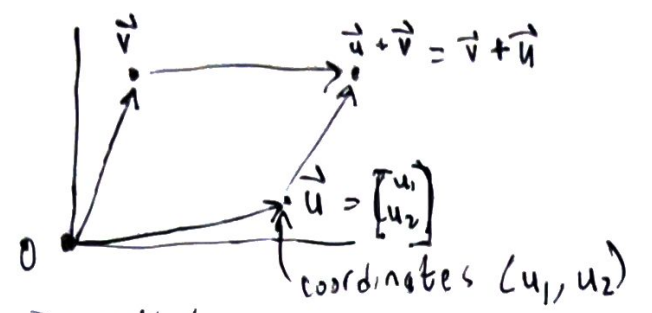
\includegraphics[width=0.5\paperwidth, center]{images/vector-addition.PNG}
		\end{figure}
	
		\item Multiplication
		\begin{itemize}
			\item scalar (real number) times vector only
			\item $c\vec{u} = c
			\begin{bmatrix}
				u_1\\
				u_2\\
				\vdots\\
				u_n
			\end{bmatrix}
			=
			\begin{bmatrix}
				cu_1\\
				cu_2\\
				\vdots\\
				cu_n
			\end{bmatrix}$
		\end{itemize}
		\begin{figure}[h!]
			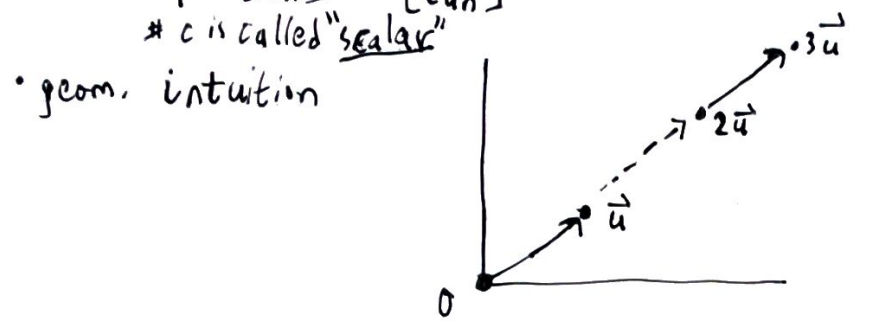
\includegraphics[width=0.8\paperwidth]{images/vector-multiplication.PNG}
		\end{figure}
	\end{itemize}
	
	\textbf{Properties}
	\begin{itemize}
		\item zero vector = $\vec{0} =
		\begin{bmatrix}
			0\\
			0\\
			\vdots\\
			0
		\end{bmatrix}$
		\item $-\vec{u} = (-1)\vec{u}$
		\item $\vec{u} + \vec{v} = \vec{v} + \vec{u}$
		\item $(\vec{u} + \vec{v}) + \vec{w} = \vec{u} + (\vec{v} + \vec{w})$
		\item $\vec{u} + \vec{0} = \vec{0} + \vec{u} = \vec{u}$
		\item $-\vec{u} + \vec{u} = \vec{0}$
		\item $(c(\vec{u} + \vec{v}) = c\vec{u} + c\vec{v}$
		\item $(c + d)\vec{u} = c\vec{u} + d\vec{u}$
		\item $c(d\vec{u}) = (cd)\vec{u}$
		\item 1$\vec{u} = \vec{u}$
	\end{itemize}
	
	\textbf{Linear Combinations}
	\begin{itemize}
		\item a \textbf{linear combination} is a vector written as the sum of other vectors
		\item the equation $\vec{y} = c_1\vec{v_1} + \ldots + c_p\vec{v_p}$
		\item $v_1,v_2,...,v_p$ are vectors $c_1,c_2,...,c_p$ are \textbf{weights}
		\item $\vec{y}$ is written as a linear combination of $v_1,v_2,...,v_p$ with weights $c_1,c_2,...,c_p$
		
		\begin{example}
			$\begin{bmatrix}
				4\\
				5
			\end{bmatrix}$
			is a linear combination of
			$\begin{bmatrix}
				1\\
				1
			\end{bmatrix}$
			and
			$\begin{bmatrix}
				2\\
				3
			\end{bmatrix}$
			because
			$\begin{bmatrix}
				4\\
				5
			\end{bmatrix}
			=
			2
			\begin{bmatrix}
				1\\
				1
			\end{bmatrix}
			+
			1
			\begin{bmatrix}
				2\\
				3
			\end{bmatrix}$.
			The weights are 2 for
			$\begin{bmatrix}
				1\\
				1
			\end{bmatrix}$
			and 1 for
			$\begin{bmatrix}
				2\\
				3
			\end{bmatrix}$.
		\end{example}
	\end{itemize}
	
	\subsection{Span}
	\begin{itemize}
		\item because of our definition of linear combinations, we have the following relation:
		
		a vector equation
		\begin{equation*}
			x_1\vec{a_1} + x_2\vec{a_2} + \ldots + x_n\vec{a_n} = \vec{b}
		\end{equation*}
		has the same solution set as the linear system with augmented matrix
		\begin{equation*}
			\begin{bmatrix}
				\vec{a_1} & \vec{a_2} & \ldots & \vec{a_n} & \vec{b}
			\end{bmatrix}
		\end{equation*}
		
		\item solving this matrix is equivalent to finding weights in a linear combination
		
		\item the \textbf{span} of a set of vectors is set of all possible linear combinations of those vectors
		
		\item if an augmented matrix $\begin{bmatrix}
			\vec{a_1} & \vec{a_2} & \ldots & \vec{a_n} & \vec{b}
		\end{bmatrix}$
		is consistent, then $\vec{b}$ is in the span of $\{\vec{a_1}, \vec{a_2}, \ldots, \vec{a_n}\}$, or, in other words, $\vec{b} \in span\{\vec{a_1}, \vec{a_2}, \ldots, \vec{a_n}\}$
		
		\item the span of two vectors is a plane
		
		\item geometric intuition:
		
		\begin{figure}[h!]
			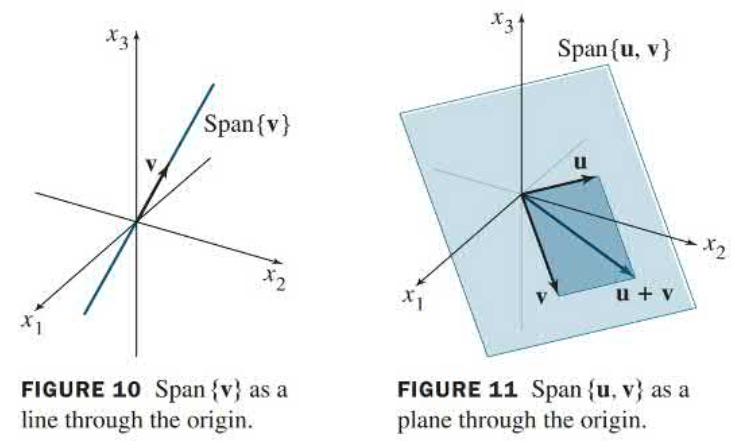
\includegraphics[width=0.5\paperwidth, center]{images/span.PNG}
		\end{figure}
	\end{itemize}
	
	\subsection{The Matrix Equation $A\vec{x} = \vec{b}$}
	\begin{itemize}
		\item fundamental idea of linear algebra is to view linear combo of vectors as product of matrix and vector (matrix vector multiplication)
		
		\item $A\vec{x}$ only defined when \# columns of A = \# entries of $\vec{x}$
		
		\item $A\vec{x}$ is a vector
		
		\begin{example}
			\begin{align*}
				\begin{bmatrix}
					1 & 2 & -1\\
					5 & 6 & 3
				\end{bmatrix}
				\begin{bmatrix}
					2\\
					7\\
					3
				\end{bmatrix}&=
				2
				\begin{bmatrix}
					1\\
					5
				\end{bmatrix}
				+ 7
				\begin{bmatrix}
					2\\
					6
				\end{bmatrix}
				+ 3
				\begin{bmatrix}
					-1\\
					3
				\end{bmatrix}\\
				&=
				\begin{bmatrix}
					2\\
					10
				\end{bmatrix}
				+
				\begin{bmatrix}
					14\\
					42
				\end{bmatrix}
				+
				\begin{bmatrix}
					-3\\
					9
				\end{bmatrix}\\
				&=
				\begin{bmatrix}
					13\\
					61
				\end{bmatrix}
			\end{align*}
		\end{example}
		
		\item See \autoref{thm:A-x-b-thm} and \autoref{thm:A-x-b-relation-thm}
		
		\item use \nameref{sec:g-j-elim} see if system is consistent or not
		
		\item Properties of $A\vec{x}$ multiplication: \autoref{thm:A-x-b-props}
	\end{itemize}
	
	\subsection{Homogenous and Nonhomogenous SoEs, and Parametric Vector Form}
	\begin{itemize}
		\item \textbf{homogenous} SoEs are SoEs hat cna be written as $A\vec{x} = \vec{0}$
		
		\item homogenous SoEs are always consistent ($\vec{a} = \vec{0}$ is always solution, which is called the \textbf{trivial solution})
		
		\item care about nontrivial solutions to the equation since we know that there is always a solution
		
		\item can write solution set of matrix equation as a vector using parametric description of solution set, known as \textbf{parametric vector form}
		
		\item to write in parametric vector form, see \nameref{sec:parametric-vector-form}
		
		\begin{example}
			The vector form of the parametric description
			\begin{align*}
				x_1 &= (4/3)x_3\\
				x_2 &= 0\\
				x_3 & \:is \:free
			\end{align*}
			is
			\begin{equation*}
				\vec{x} =
				\begin{bmatrix}
					(4/3)x_3\\
					0\\
					x_3
				\end{bmatrix}
				= x_3
				\begin{bmatrix}
					4/3\\
					0\\
					1
				\end{bmatrix}
			\end{equation*}
		\end{example}
		
		\item Non-homogenous SoEs have same parametric vector form solution as $A\vec{x} = \vec{0}$, but with extra vector added that comes from $\vec{b}$ (see \autoref{thm:non-homo-thm})
	\end{itemize}
	
	\subsection{Linear Dependence}
	\begin{itemize}
		\item see definitions for \textbf{linear independence and linear dependence}
		
		\item columns of a matrix $A$ are linearly indep. $\Leftrightarrow \mateqaxo$ has only trivial solution
		
		\item see \nameref{sec:lin-indep-check}, \autoref{thm:lin-dep-thm}, \autoref{thm:lin-dep-thm-p-gt-n}, and \autoref{thm:lin-dep-thm-zero-vec}
	\end{itemize}
	
	\subsection{Transformations}
	\begin{itemize}
		\item a transformation $T$ is a function that maps a vector $\vec{x}$ to a vector $A\vec{x}$
		
		\item $T(\vec{x}) = A\vec{x}$ for a matrix $A$. Notation: $T: \mathbb{R}^n \rightarrow \mathbb{R}^m$
		
		\item $T$ has a \textbf{domain} and \textbf{co-domain}. For a $\vec{x}$, the \textbf{image} of $\vec{x}$ is $T(\vec{x}) = A\vec{x}$, and the \textbf{range} is all possible images under $T$.
		
		\begin{figure}[h!]
			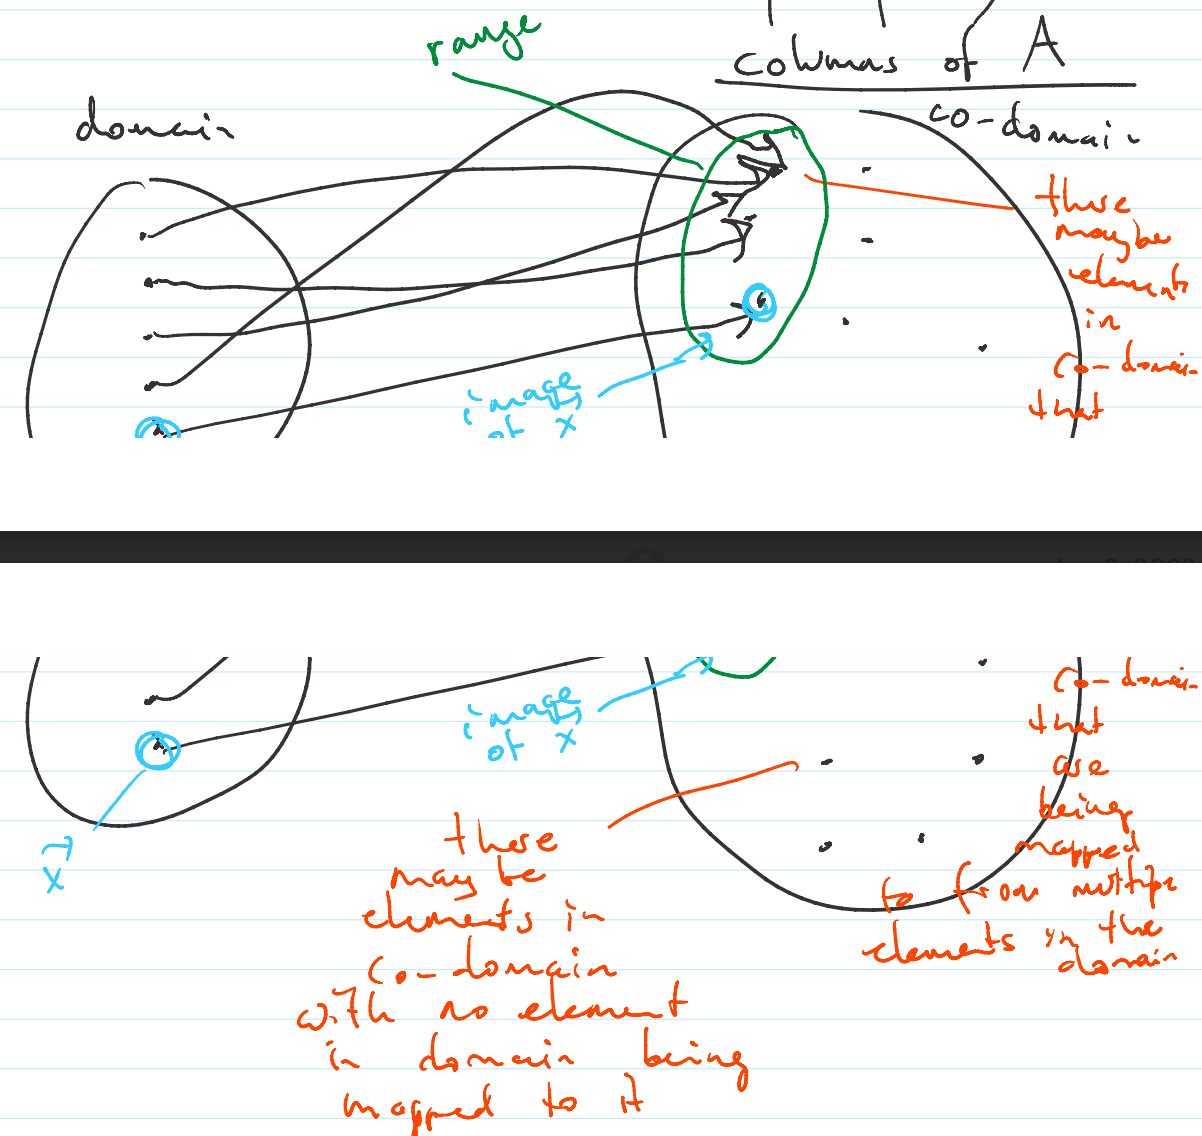
\includegraphics[width=0.5\paperwidth, center]{images/lin-transforms-diagram.PNG}
		\end{figure}
		
		\item $\vec{x} \mapsto A\vec{x}$ means $\vec{x}$ maps to $A\vec{x}$
		
		\item Properties of linear transformations:
		\begin{enumerate}
			\item $T(\vec{u} + \vec{v}) = T(\vec{u}) + T(\vec{v})$
			
			\item $T(c\vec{u}) = cT(\vec{u})$
		\end{enumerate}
		
		\item these properties lead to the following facts:
		\begin{enumerate}
			\item $T(\vec{0}) = \vec{0}$ (though the $\vec{0}$ vectors can be in different spaces)
			
			\item $T(c\vec{u} + d\vec{v}) = cT(\vec{u}) + dT(\vec{v})$.
			
			\item $T(\lincombo{c}{\vec{v}}{p}{p}) = \finiteadd{c_1T(\vec{v_1})}{c_2T(\vec{v_2})}{c_pT(\vec{v_p})}$
		\end{enumerate}
		
		\item linear transformations can also be \textbf{onto} (all points in co-domain have at least one arrow pointing in) and/or \textbf{one-to-one} (no points in co-domain with more than 1 arrow pointing in)
		
		\item See \autoref{thm:lin-trans-unique-mat-thm}, \autoref{thm:lin-trans-one-to-one-thm}, \autoref{thm:onto-and-one-to-one-thm}
	\end{itemize}
	
	\subsection{Key Matrices and Matrix Algebra}
	\begin{itemize}
		\item think of matrices as structure with vectors as columns
		
		\begin{flalign*}
			A &=
			\begin{bmatrix}
				\vec{a_1} & \vec{a_2} & \ldots & \vec{a_n}
			\end{bmatrix}&&\\
			&=
			\begin{bmatrix}
				a_{11} & a_{11} & \ldots & a_{1n}\\
				a_{21} & a_{22} & \ldots & a_{2n}\\
				\vdots\\
				a_{m1} & a_{m2} & \ldots & a_{mn}
			\end{bmatrix}
		\end{flalign*}
		
		\item \textbf{diagonal entries} are $a_{11}, a_{22}, a_{33}, \ldots$, which form \textbf{main diagonal} of $A$.
		
		\item \textbf{diagonal matrix} (only diagonal entries are nonzero)
		$\begin{bmatrix}
			3 & 0 & 0\\
			0 & 3 & 0\\
			0 & 0 & 3
		\end{bmatrix}$,
		\textbf{identity matrix} (diagonal matrix where diagonal entries are 1)
		$\begin{bmatrix}
			1 & 0 & 0\\
			0 & 1 & 0\\
			0 & 0 & 1
		\end{bmatrix}$,
		and \textbf{zero matrix} (all entries 0)
		$\begin{bmatrix}
			0 & 0 & 0\\
			0 & 0 & 0\\
			0 & 0 & 0
		\end{bmatrix}$
		are also important to know about
		
		\item Addition: 
		\begin{itemize}
			\item $A + B$ only defined if $A$ and $B$ are the same size
			
			\item result is sum of corresponding entries in $A$ and $B$
		\end{itemize}
		
		\item Scalar Multiplication: 
		\begin{itemize}
			\item $rA =
			\begin{bmatrix}
				r\vec{a_1} & r\vec{a_2} & \ldots r\vec{a_n}
			\end{bmatrix}$
		\end{itemize}
		
		\item See \autoref{thm:mat-add-sclmult-props} for properties of the operations
		
		\item Matrix Multiplication:
		\begin{itemize}
			\item only defined if \# rows of $B$ = \# columns of $A$
			
			\item $AB =
			\begin{bmatrix}
				A\vec{b_1} & A\vec{b_2} & \ldots & A\vec{b_p}
			\end{bmatrix}$
			
			\item if $A$ is $m \times n$ matrix and $B$ is $n \times p$ matrix, size of $AB$ = $m \times p$
			
			\item ORDER MATTERS!!!!! ($AB \neq BA$ generally, even if both multiplications are defined)
			
			\item if $AB = 0$ one cannot conclude that $A = 0$ or $B = 0$
			
			\item See \autoref{thm:mat-mult-props} for properties of matrix multiplication
		\end{itemize}
		
		\item Powers of a square matrix:
		\begin{itemize}
			\item $A^k = A \times A \times A \times \ldots \times A$ (k times)
			
			\item $A^0 = I$
		\end{itemize}
		
		\item Transpose:
		\begin{itemize}
			\item transpose of matrix is matrix where rows of original matrix become columns of the new matrix and vice versa
			
			\begin{example}
				$\begin{bmatrix}
					1 & 7 & 9\\
					6 & 4 & 2\\
					3 & 4 & 3
				\end{bmatrix}^T
				=
				\begin{bmatrix}
					1 & 6 & 3\\
					7 & 4 & 4\\
					9 & 2 & 3
				\end{bmatrix}$
			\end{example}
			
			\item See \autoref{thm:mat-transpose-props} for properties of matrix transposes
		\end{itemize} 
	\end{itemize}
	
	\subsection{Invertible Matrices}
	\begin{itemize}
		\item invertibility only applies to square matrices, so matrices in this section are all square ($n \times n$)
		
		\item a matrix is invertible if there exists a matrix $C$ such that $AC = I$ and $CA = I$. $C$ is the inverse of $A$ (denoted as $A^{-1}$) in this case.
		
		\item non-invertible matrices are sometimes called \textbf{singular matrices}, and invertible matrices are sometimes called \textbf{nonsingular matrices}.
		
		\item the matrix 
		$\begin{bmatrix}
			0
		\end{bmatrix}$
		is not invertible
		
		\item see \autoref{thm:two-by-two-mat-invert-thm} and \autoref{thm:invert-mat-unique-soln-thm} and \autoref{thm:invert-mat-algebra}
		
		\item To find inverse of matrix: see \nameref{sec:mat-inverse}
		
		\item IMPORTANT THEOREM: \autoref{thm:imt-thm}
		
		\item a transformation $T$ is invertible if there exists if there exists a transformation $S$ such that
		\begin{enumerate}[i.]
			\item $S(T(\vec{x})) = \vec{x}$ for all $\vec{x}$ in the domain of $T$
			\item $T(S(\vec{b})) = \vec{b}$ for all $\vec{b}$ in the domain of $S$
		\end{enumerate}
		
		\item see \autoref{thm:invertible-trans-thm}
	\end{itemize}
	
	\subsection{LU Factorization}
	\begin{itemize}
		\item factorization that makes it easier to solve for $\mateqaxb$ faster
		
		\item $L and U$ have a special structure:
		\begin{enumerate}[a.]
			\item $L$ is "lower triangular" with 1s on diagonal
			
			\item $U$ is the echelon form of $A$ (so "upper triangular", 0s below diagonal)
			
			\begin{equation}
				A =
				\underset{L}
				{\begin{bmatrix}
						1 & 0 & 0 & 0\\
						* & 1 & 0 & 0\\
						* & * & 1 & 0\\
						* & * & * & 1
				\end{bmatrix}}
				\underset{U}
				{\begin{bmatrix}
						\blacksquare & * & * & * & *\\
						0 & \blacksquare & * & * & *\\
						0 & 0 & 0 & \blacksquare & *\\
						0 & 0 & 0 & 0 & 0
				\end{bmatrix}}
			\end{equation}
		\end{enumerate}
		
		\item Method: see \nameref{sec:lu-factorization} and \nameref{sec:axb-solve-lu-factor}
	\end{itemize}
	
	\subsection{Vector Spaces and Subspaces}
	\begin{itemize}
		\item a \textbf{vector space} is nonempty set, $V$, of objects (called vectors). Two operations can be performed on these vectors: addition, scalar multiplication
		
		\item 10 Vector axioms for vector space $V$, vectors $\vec{u}, \vec{v}, \vec{w}$, scalars $c and d$:
		
		\begin{enumerate}
			\item $\vec{u} + \vec{v} \in V$
			\item $\vec{u} + \vec{v} = \vec{v} + \vec{u}$
			\item $(\vec{u} + \vec{v}) + \vec{w} = \vec{u} + (\vec{v} + \vec{w)}$
			\item there is $\vec{0} \in V$ such that $\vec{u} + \vec{0} = \vec{u}$ for all $\vec{u} \in V$
			\item there is $\vec{-u} \in V$ such that $\vec{u} + (\vec{-u}) = \vec{0}$
			\item $c\vec{u} \in V$
			\item $c(\vec{u} + \vec{v}) = c\vec{u} + c\vec{v}$
			\item $(c + d)\vec{u} = c\vec{u} + d\vec{u}$
			\item $c(d\vec{u}) = (cd)\vec{u}$
			\item $1\vec{u} = \vec{u}$
		\end{enumerate}
		
		\item from the axioms, we have
		\begin{enumerate}
			\item $0\vec{u} = \vec{0}$
			\item $c\vec{0} = \vec{0}$
			\item $\vec{-u} = (-1)\vec{u}$
		\end{enumerate}
		
		\item polynomials of a degree $n$ can be a vector space $\mathbb{P}^n$
		
		\item \textbf{subspace} of vector space $V$ is a subset, $H$, of $V$ that has three properties:
		\begin{enumerate}
			\item $H$ is a nonempty subset of $V$ $\Leftrightarrow \vec{0} \in H$
			\item $\vec{u}, \vec{v} \in H$ implies $\vec{u} + \vec{v} \in H$ (closed under addition)
			\item $\vec{u}\in H$ and scalar $c$ implies $c\vec{u} \in H$ (closed under multiplication)
		\end{enumerate}
		
		\item a subspace is vector space, vector space is subspace
		
		\item see \autoref{thm:span-subspace-thm}
	\end{itemize}
	
	\subsection{The Fundamental Spaces}
	Given an $m \times n$ matrix $A$, and a linear transformation $T$:
	\begin{description}[style=nextline]
		\item[null space] the solution set to $\mateqaxo$. denoted by Nul$A$. Nul$A = \{\vec{x}: \mateqaxo\}$ is the fancy math way of saying it. Nul$A$ is a vector space, because it is a subspace of $\mathbb{R}^n$.
		
		\item[column space] the set of all linear combinations of the columns of $A$. denoted by Col$A$ If $A =
		\begin{bmatrix}
			\vec{a_1} & \ldots & \vec{a_n}
		\end{bmatrix}$
		then Col$A = \{\vec{b} : \mateqaxb for some \vec{x}\} =$ Span$\finitevecsset{a}{n}$. It is a subspace of $\mathbb{R}^m$.
		
		\item[row space] the set of all linear combinations of the rows of A. denoted by Row$A$. Row$A$ = Col$A^T$.
		
		\item[kernel] the set of all $\vec{u}$ such that $\mateq{T}{(\vec{x})}{\vec{0}}$. Kernel($T$) = $\{\vec{x}: T(\vec{x}) = \vec{0}\} =$ Nul$A$
	\end{description}
	
	\begin{itemize}
		\item see \nameref{sec:solve-fund-spcs} to solve for these mathematically
	\end{itemize}
	
	\subsection{Bases, Bases for Fundamental Spaces, Change of Bases}
	\begin{itemize}
		\item a \textbf{basis} is a linearly independent set of vectors that span a subspace
		
		\item If $H$ is a subspace of $V$, a set of vectors $B \subseteq V$ is a \textbf{basis} for $H$ means
		\begin{enumerate}[i.]
			\item $B$ is a linearly independent set
			\item $H =$ span$\{B\}$
		\end{enumerate}
		
		\item see \autoref{thm:lin-dep-vec-set-thm}, \autoref{thm:spanning-set-thm}, \autoref{thm:basis-col-space-thm},
		\autoref{thm:row-space-equiv-thm}
		
		\item see \nameref{sec:solve-bases-fund-spcs}
	\end{itemize}
	
	\subsection{Coordinate Systems}
	\begin{itemize}
		\item see \autoref{thm:uniq-rep-thm}
		
		Given $\vec{x} = \finiteadd{c_1\vec{b_1}}{c_2\vec{b_2}}{c_n\vec{b_n}}$, where $B = \finitevecsset{b}{n}$:
		
		\item the \textbf{coordinates} of $\vec{x}$ relative to $B$ are the weights $\finitevecs{c}{n}$ ($\basiscoordvec{x}{B}
		=
		\begin{bmatrix}
			\vec{c_1}\\
			\vec{c_2}\\
			\vdots\\
			\vec{c_n}\\
		\end{bmatrix}$)
		
		\item the \textbf{change of coordinates} matrix is a matrix such that when the coordinates of $\vec{x}$ relative to $B$ is multiplied by it, $\vec{x}$ is produced. It is denoted $P_B$ ($P_B =
		\begin{bmatrix}
			b_1 & b_2 & \ldots &b_n
		\end{bmatrix}$)
		
		\item $\vec{x} = P_B\basiscoordvec{x}{B}$, $P^{-1}_B\vec{x} = \basiscoordvec{x}{B}$
		
		\item $P^{-1}_B$ is change-of-coordinates matrix from standard basis to $B$
		
		\item $\vec{x} \mapsto \basiscoordvec{x}{B}$ is one-to-one and onto linear transformation
		
		\item $\mateq{T}{(\vec{x})}{\basiscoordvec{x}{B}}$ is a linear transformation, one-to-one, onto
		
		\item an \textbf{isomorphism} is a linear transformation that is both one-to-one and onto.
		
		\item \textbf{change-of-coordinate-matrix} is a square matrix that converts from coordinates in one base to another. denoted $\chngbasismat{B}{C}$ for bases $B, C$
		
		\item Given base $B = \finitevecsset{b}{n}$ and $C = \finitevecsset{c}{n}$ are bases of vector space $V$:
		\begin{equation*}
			\basiscoordvec{x}{C} = \chngbasismat{B}{C}\basiscoordvec{x}{B}
		\end{equation*}
		
		\begin{equation*}
			\chngbasismat{B}{C}
			=
			\begin{bmatrix}
				\basiscoordvec{b_1}{C} & \basiscoordvec{b_2}{C} & \ldots & \basiscoordvec{b_n}{C}
			\end{bmatrix}
		\end{equation*}
		
		\item $(\chngbasismat{B}{C})^{-1} = \chngbasismat{C}{B}$
		
		\item $\begin{bmatrix}
			\vec{c_1} & \vec{c_2} & \vdots & \vec{b_1} & \vec{b_2}
		\end{bmatrix}
		\sim
		\begin{bmatrix}
			I & \vdots & \chngbasismat{B}{C}
		\end{bmatrix}$
	\end{itemize}
	
	\subsection{Dimensions}
	\begin{itemize}
		\item \textbf{dimension}: number of vectors in a basis of a vector space $V$ (provided there are a finite number of vectors). denoted dim($V$).
		
		\item see \autoref{thm:vec-spc-same-num-vec-thm}, \autoref{thm:vec-spc-lin-dep}
		
		\item dim($\vec{0}$) = 0
		
		\item rank$A$ = dim(Col$A$) = dim(Row$A$) = number of pivot columns of $A$ = number of rows with a pivot in EF of $A$
		
		\item dim(Nul$A$) = nullity of A = \# of non pivot columns in $A$.
		
		\item see \autoref{thm:rank-nul-thm}, \autoref{thm:imt-thm} (adds some new content with this knowledge), \autoref{thm:vec-spc-dim-thm}
	\end{itemize}
	
	\subsection{Determinants}
	\begin{itemize}
		\item the following only applies for \textbf{square} matrices
		
		\item \textbf{determinant} is the volume of a geometric object with edges as the rows of $A$
		
		\item det$A = 0 \Leftrightarrow A$ is not invertible
		
		\item Properties of determinants:
		\begin{enumerate}
			\item det$I$ = 1
			\item if $A$ has 2 rows that are the same, det$A$ = 0
			\item If a matrix has a row of 0s, then det$A$ = 0
			\item replacement operations do not change determinant
			\item the determinant of a matrix $B$ obtained by a row interchange on a matrix is $-$det$A$
			\item scaling operation by a scalar $k$ makes the determinant $k$det$S$
			\item the determinant of a diagonal or triangular matrix is the product of its diagonal entries
			\item det$A$ = det$A^T$
			\item det$AB$ = (det$A$)(det$B$), det$A^2$ = $(\text{det}A)^2$
			\item det$A^{-1}$ = $\frac{1}{\text{det}A}$
		\end{enumerate}
		
		\item det($
		\begin{bmatrix}
			a & b\\
			c & d\\
		\end{bmatrix}$) $= ad - bc$
		
		\item to solve for determinant of matrix, see \nameref{sec:co-factor-exp}
	\end{itemize}
	
	\subsection{Entering the Eigenarena}
	\begin{itemize}
		\item the following only applies to \textbf{square} matrices
		
		\item \textbf{eigenvalues} (denoted $\lambda$) are scalars that fulfill the $\eigeneq$ (basically saying that multiplying $A$ by $\vec{x}$ gives a scaled version of $\vec{x}$), and \textbf{eigenvectors} are the $\vec{x}$ that correspond to the eigenvalue in the equation
		
		\item if given an eigenvalue ($\lambda$) of a matrix $A$, finding eigenvectors corresponding to $\lambda$ corresponds to solving $(A - \lambda I)\vec{x} = \vec{0}$. the solution set to this system is called the \textbf{eigenspace} corresponding to $\lambda$ (which is essentially Nul$A - \lambda I$)
		
		\item eigenvalues of triangular matrix are the values on its main diagonal
		
		\item see \autoref{thm:eigen-vec-lin-indep-thm}
		
		\item \textbf{characteristic equation} of $A$ is $\chareq$. To find eigenvalues of $A$, solve this equation
		
		\item to find eigenspaces and eigenvalues, see \nameref{sec:finding-eigenspcs-and-eigenvals}
		
%		TODO: make a command for printing a finite set of fractions
		\item if $A$ has eigenvalues $\finitevecs{\lambda}{n}$, then $A^{-1}$ has eigenvalues $\frac{1}{\lambda_1}, \ldots \frac{1}{\lambda_n}$
		
		\item see \autoref{thm:zero-eigenval-invertibility-thm}
		
		\item $A$ and $B$ are \textbf{similar} means there exists an invertible matrix $P$ such that $A = PBP^{-1}$
		
		\item see \autoref{similar-mat-char-eq-thm}
	\end{itemize}
		
	\subsubsection{Transformations in the Eigenarena}
	\begin{itemize}
		\item $\lambda$ and $\vec{x}$ are an eigenvalue and eigenvector of $T$ means $T(\vec{x}) = \lambda\vec{x}$
		
		\item to find matrix for $T$ relative to basis $B$:
		\begin{equation*}
			M =
			\begin{bmatrix}
				\basiscoord{T(\vec{b_1})}{B} & \basiscoord{T(\vec{b_2})}{B} & \ldots \basiscoord{T(\vec{b_n})}{B}
			\end{bmatrix}
		\end{equation*}
	\end{itemize}
	
	\subsection{Diagonalization (another factorization)}
	\begin{itemize}
		\item the following only applies to \textbf{square} matrices
		
		\item a matrix $A$ is \textbf{diagonalizable} if it is similar to a diagonal matrix $D$, which is the same thing as saying there exists an invertible matrix $P$ such that $A = PDP^{-1}$
		
		\item if a matrix is diagonalizable, it is very easy to find $A^k$
		
		\item see \autoref{thm:diagonlization-thm}, \autoref{thm:eigenvec-diagonlization-thm}
		
		\item to diagonlize a matrix, see \nameref{sec:diagonlizing-matrices}
		
		\item $A^k = PD^kP^{-1}$
	\end{itemize}
	
	\subsection{Power Method}
	\begin{itemize}
		\item method to find approximate eigenvalues and eigenvectors using a computer
		
		\item to estimate a strictly dominant eigenvalue \nameref{sec:power-method}
	\end{itemize}
	
	\subsection{Complex Eigenvalues}
	\begin{itemize}
		\item eigenvalues can unfortunately be complex numbers
		
		\item matrices with complex eigenvalues correspond to rotations in terms of transformations
		
		\item $A^k$ will have real eigenvalues if $A$ has real eigenvalues
		
		\item complex numbers have a real part and imaginary part. Re$(z)$ represents the real part of the complex number $z$, and Im$(z)$ is the imaginary part. $z =$ Re$(z)$ $+$ $i$Im$(z)$
		
		\item \textbf{Properties of complex number algebra} ($B$ is an $m \times n$ matrix, $\bar{B}$ is a matrix whose entries are the complex conjugates of entries in $B$, $r$ is a complex number, $\vec{x}$ is a vector):
		
		\begin{itemize}
			\item $\overline{r\vec{x}} = \overline{r}\overline{\vec{x}}$
			
			\item $\overline{B\vec{x}} = \overline{B}\overline{\vec{x}}$
			
			\item $\overline{BC} = \overline{B}\overline{C}$
			
			\item $\overline{rB} = \overline{r}\overline{B}$
		\end{itemize}
		
		\item because of these properties, if $\lambda =$ Re$(z)$ $+$ $i$Im$(z)$, then $\bar{\lambda} =$ Re$(z)$ $-$ $i$Im$(z)$ is also an eigenvalue of $A$, where $\bar{\lambda}$ is the complex conjugate of $A$
		
		\item If $A$ is real $2 \times 2$ matrix with complex eigenvalues $\lambda_1 = a + ib$ and $\lambda_2 = a - ib$ ($b \neq 0$) and corresponding eigenvector for $\lambda_1$ $\vec{v}$, then:
		\begin{align*}
			A &= PCP^{-1}\\
			C &=
			\begin{bmatrix}
				a & -b\\
				b & a
			\end{bmatrix}\\
			P &=
			\begin{bmatrix}
				\text{Re}(\vec{v}) & \textbf{Im}(\vec{v})
			\end{bmatrix}
		\end{align*}
	\end{itemize}
	\newpage
	
	\section{Important Theorems}
	\begin{theorem}
		Each matrix is row equivalent to one and only one reduced echelon matrix.
	\end{theorem}
	
	\begin{theorem}
		\label{thm:A-x-b-thm}
		When A is $m \times n$ matrix with columns $a_1,\ldots,a_n$, and $\vec{b}$ in $\mathbb{R}^m$,
		\begin{equation*}
			\mateqaxb
		\end{equation*}
		has same solution set as
		\begin{equation*}
			x_1\vec{a_1} + x_2\vec{a_2} + \ldots + x_n\vec{a_n} = \vec{b}
		\end{equation*}
		which has same solution set as 
		\begin{equation*}
			\begin{bmatrix}
				\vec{a_1} & \vec{a_2} & \ldots & \vec{a_n} & \vec{b}
			\end{bmatrix}
		\end{equation*}
	\end{theorem}
	
	\begin{theorem}
		\label{thm:A-x-b-relation-thm}
		Let $A$ be an $m \times n$ matrix (coefficient matrix). Then the following statements are logically equivalent.
		That is, for a particular $A$, either they are all true statements or they are all false.
		\begin{enumerate}[a.]
			\item For each $\vec{b}$ in $\mathbb{R} ^ m$, the equation $A\vec{x} = \vec{b}$ has a solution.
			
			\item Each $\vec{b}$ in $\mathbb{R} ^ m$ is a linear combination of the columns of A.
			
			\item The columns of $A$ span $\mathbb{R} ^ m$.
			
			\item A has a pivot position in every row.
		\end{enumerate}
	\end{theorem}
	
	\begin{theorem}
		\label{thm:A-x-b-props}
		Let $A$ be an $m \times n$ matrix, $\vec{u}$ and $\vec{v}$ are vectors in $\mathbb{R}^n$, and $c$ is a scalar, then:
		
		\begin{enumerate}[a.]
			\item $A(\vec{u} + \vec{v}) = A\vec{u} + A\vec{v}$
			
			\item $A(c\vec{u}) = c(A\vec{u})$
		\end{enumerate}
	\end{theorem}
	
	\begin{theorem}
		\label{thm:non-homo-thm}
		Suppose the equation $A\vec{x} = \vec{b}$ is consistent for some given $\vec{b}$, and let $\vec{p}$ be a
		solution. Then the solution set of $A\vec{x} = \vec{b}$ is the set of all vectors of the form
		$\vec{w} = \vec{p} + \vec{v_h}$, where $\vec{v_h}$ is any solution of the homogeneous equation $A\vec{x} = \vec{0}$.
	\end{theorem}
	
	\begin{theorem}
		\label{thm:lin-dep-thm}
		
		A set of vectors $\finitevecsset{\vec{v}}{p}$ is linearly dependent if one of the vectors is a linear combination of the others. ($v_j \in span{v_1, v_2,\ldots,v_{j-1}, v_{j+1},\ldots,v_p}$) for some $j$.
	\end{theorem}
	
	\begin{theorem}
		\label{thm:lin-dep-thm-p-gt-n}
		
		A set of vectors $\finitevecsset{\vec{v}}{p}$ is linearly dependent if there are more vectors than entries in each vector. Any set $\finitevecsset{\vec{v}}{p}$ in $\mathbb{R}^n$ is linearly dependent if $p > n$.
	\end{theorem}
	
	\begin{theorem}
		\label{thm:lin-dep-thm-zero-vec}
		
		A set of vectors $\finitevecsset{\vec{v}}{p}$ is linearly dependent if it contains the zero vector.
	\end{theorem}
	
	\begin{theorem}
		\label{thm:lin-trans-unique-mat-thm}
		Given a linear transformation $T: \mathbb{R}^n \rightarrow \mathbb{R}^m$ there exists a unique matrix A such that
		\begin{equation*}
			T(\vec{x}) = A\vec{x}
		\end{equation*}
		namely
		\begin{equation*}
			A =
			\begin{bmatrix}
				T(\vec{e_1}) & T(\vec{e_2}) & \ldots & T(\vec{e_n})
			\end{bmatrix}
		\end{equation*}
		where
		\begin{equation*}
			\vec{e_1} =
			\begin{bmatrix}
				1\\
				0\\
				0\\
				\vdots\\
				0
			\end{bmatrix}
			\vec{e_2} =
			\begin{bmatrix}
				0\\
				1\\
				0\\
				\vdots\\
				0
			\end{bmatrix}
			\vec{e_j} =
			\begin{bmatrix}
				0\\
				\vdots\\
				0\\
				1 \leftarrow j^{th} entry\\
				\vdots\\
				0\\
				\vdots\\
				0
			\end{bmatrix}
		\end{equation*}
		$\finitevecs{\vec{e}}{j}$ are known as \textbf{standard basis vectors}. The matrix A is the \textbf{standard matrix for the linear transformation T}.
	\end{theorem}
	
	\begin{theorem}
		\label{thm:lin-trans-one-to-one-thm}
		
		Given a linear transformation $T: \mathbb{R}^n \rightarrow \mathbb{R}^m$, T is one-to-one exactly when $\mateq{T}{(\vec{x})}{\vec{0}}$ has only the trivial solution.
	\end{theorem}
	
	\begin{theorem}
		\label{thm:onto-and-one-to-one-thm}
		
		Given a linear transformation $T: \mathbb{R}^n \rightarrow \mathbb{R}^m$ with standard matrix A:
		\begin{enumerate}[a.]
			\item $T$ is onto $\Leftrightarrow$ span of columns of $A = \mathbb{R}^m$.
			
			\item $T$ is one-to-one $\Leftrightarrow \mateqaxo$ only has trivial solution, $\Leftrightarrow$ columns of $A$ are linearly independent.
		\end{enumerate}
	\end{theorem}
	
	\begin{theorem}
		\label{thm:mat-add-sclmult-props}
		
		Given matrices $A, B, C$ of the same size, and $r, s$ are scalars:
		\begin{enumerate}[a.]
			\item $A + B = B + A$
			\item $(A + B) + C = A + (B + C)$
			\item $A + 0 = A$
			\item $r(A + B) = rA + rB$
			\item $(r + s)A = rA + sA$
			\item $r(sA) = (rs)A$
		\end{enumerate}
	\end{theorem}
	
	\begin{theorem}
		\label{thm:mat-mult-props}
		
		Given $A, B, C$ matrices such that sums and products below are defined:
		
		\begin{enumerate}[a.]
			\item $A(BC) = (AB)C$
			\item $A(B + C) = AB + AC$
			\item $(B + C)A = BA + CA$
			\item $r(AB) = (rA)B = A(rB)$
			\item $IA = A = AI$
		\end{enumerate}
	\end{theorem}
	
	\begin{theorem}
		\label{thm:mat-transpose-props}
		
		Given a matrix $A$:
		\begin{enumerate}[a.]
			\item $(A^T)^T = A$
			\item $(A + B)^T = A^T + B^T$
			\item $(rA)^T = rA^T$
			\item $(AB)^T = B^TA^T$
		\end{enumerate}
	\end{theorem}
	
	\begin{theorem}
		\label{thm:two-by-two-mat-invert-thm}
		Given $A
		=
		\begin{bmatrix}
			a & b\\
			c & d
		\end{bmatrix}$,
		if $ad - bc \neq 0$ then $A$ is invertible and $A^{-1} = \frac{1}{ad-bc}
		\begin{bmatrix}
			d & -b\\
			-c & a
		\end{bmatrix}$
	\end{theorem}
	
	\begin{theorem}
		\label{thm:invert-mat-unique-soln-thm}
		
		If $A$ is invertible $n \times n$ matrix, then for every $\vec{b}$ in $\mathbb{R}^n$, $\mateqaxb$ has the unique solution $\vec{x} = A^{-1}\vec{b}$.
	\end{theorem}
	
	\begin{theorem}
		\label{thm:invert-mat-algebra}
		
		Given $A, B$ invertible matrices, then
		\begin{enumerate}[a.]
			\item $A^{-1}$ is also invertible and $(A^{-1})^{-1} = A$
			
			\item $AB$ is also invertible and $(AB)^{-1} = B^{-1}A^{-1}$
			
			\item $A^T$ is also invertible and $(A^T)^{-1} = (A^{-1})^T$
		\end{enumerate}
	\end{theorem}
	
%	TODO: decide if unique theorem names should have their own environment or not
	\begin{theorem}[\textbf{Invertible Matrix Theorem}]
		\label{thm:imt-thm}
		If $A$ is an $n \times n$ matrix, then the following statements are equivalent. That
		is, for a given $A$, the statements are either all true or all false.
		
		\begin{enumerate}[a.]
			\item $A$ is an invertible matrix
			\item $\mateqaxb$ has unique solution for every $\vec{b} \in \mathbb{R}^n$.
			\item $A$ has $n$ pivot positions, and a pivot position in every row and column. (because $A$ is square)
			\item $A$ has reduced echelon form $I$
			\item $\mateqaxo$ only has trivial solution
			\item the columns of $A$ are linearly independent
			\item columns of $A$ span $\mathbb{R}^n$
			\item $A^T$ is invertible
			\item the transformation $\vec{x} \mapsto A\vec{x}$ is onto
			\item the transformation $\vec{x} \mapsto A\vec{x}$ is one-to-one
			\item there exists an $n \times n$ matrix $C$ such that $\mateq{C}{A}{I}$
			\item there exists an $n \times n$ matrix $D$ such that $\mateq{A}{D}{I}$
			\item The columns of $A$ form a basis of $\mathbb{R}^n$
			\item Col$A = \mathbb{R}^n$
			\item rank$A = n$
			\item nullity$A = 0$
			\item Nul$A = \{\vec{0}\}$
		\end{enumerate}
	\end{theorem}
	
	\begin{theorem}
		\label{thm:invertible-trans-thm}
		A linear transformation $T: \mathbb{R}^n \rightarrow \mathbb{R}^n$ with standard matrix $A$ is invertible $\Leftrightarrow A$ is an invertible matrix. In that case, $\vec{b} \mapsto A^{-1}\vec{b}$ is the inverse function of $T$.
	\end{theorem}
	
	\begin{theorem}
		\label{thm:span-subspace-thm}
		If $\finitevecs{\vec{v}}{p}$ are in a vector space $V$, then $Span\finitevecsset{\vec{v}}{p}$ is a subspace of $V$.
	\end{theorem}
	
	\begin{theorem}
		\label{thm:lin-dep-vec-set-thm}
		$\finitevecsset{v}{p}$ ($p \geq 2$) is linearly dependent $\Leftrightarrow$ one of the vectors is a linear combination of the others
	\end{theorem}
	
	\begin{theorem}[The Spanning Set Theorem]
		\label{thm:spanning-set-thm}
		Given $H$ = span$\finitevecsset{\vec{v}}{p}$ we can repeatedly find a vector that is a linear combination of the others and delete this vector from the generating set until we have a linearly independent set of vectors that still spans $S$.
	\end{theorem}
	
	\begin{theorem}
		\label{thm:basis-col-space-thm}
		The pivot columns of matrix $A$ form a basis for Col$A$.
	\end{theorem}
	
	\begin{theorem}
		\label{thm:row-space-equiv-thm}
		The row space of a matrix does not change after performing one row operation. (Row$A$ = Row$B$ if $B$ can be obtained from $A$ by performing 1 row operation)
	\end{theorem}
	
	\begin{theorem}[Unique Representation Theorem]
		\label{thm:uniq-rep-thm}
		Given $B = \finitevecsset{b}{n}$ be a basis for vector space $V$. For any $\vec{x} \in V$ there is a unique set of scalars $\finitevecs{c}{n}$ such that $\vec{x} = \finiteadd{c_1\vec{b_1}}{c_2\vec{b_2}}{c_n\vec{b_n}}$
	\end{theorem}
	
	\begin{theorem}
		\label{thm:vec-spc-lin-dep}
		$V$ vector space, with basis $B = \finitevecs{\vec{b}}{n}$: Any set of vectors in $V$ with more than $n$ vectors ($n =$ \# vectors in $B$) is linearly dependent.
	\end{theorem}
	
	\begin{theorem}
		\label{thm:vec-spc-same-num-vec-thm}
		Every basis for vector space $V$ has same \# of vectors.
	\end{theorem}
	
	\begin{theorem}[Rank-Nullity Theorem]
		\label{thm:rank-nul-thm}
		rank$A$ + nullity of $A = n$
	\end{theorem}
	
	\begin{theorem}
		\label{thm:vec-spc-dim-thm}
		Given vector space $V$, dim$V$ = p,
		\begin{enumerate}[a.]
			\item Any linearly independent set of size $p$ is a basis for $V$.
			
			\item Any set of $p$ vectors that spans $V$ is a basis for $V$.
		\end{enumerate}
	\end{theorem}
	
	\begin{theorem}
		\label{thm:eigen-vec-lin-indep-thm}
		Given distinct eigenvalues $\finitevecs{\lambda}{p}$ with eigenvectors $\finitevecs{\vec{x}}{p}$, $\finitevecsset{\vec{x}}{p}$ is linearly independent.
	\end{theorem}
	
	\begin{theorem}
		\label{thm:zero-eigenval-invertibility-thm}
		$A$ is invertible $\Leftrightarrow$ 0 is not an eigenvalue of $A$.
	\end{theorem}
	
	\begin{theorem}
		\label{similar-mat-char-eq-thm}
		Similar matrices have same characteristic equation and same eigenvalues
	\end{theorem}
	
	\begin{theorem}
		\label{thm:diagonlization-thm}
		$n \times n$ matrix $A$ is diagonlizable $\Leftarrow$ there are $n$ eigenvectors of $A$ that are linearly independent. $P$ can be constructed using these eigenvectors as columns, and $D$ can be constructured by putting the corresponding eigenvalues of $A$ on the diagonal (in the same order as the eigenvectors). To visualize this:
		\begin{equation*}
			A =
			\underset{P}{
				\begin{bmatrix}
					\vec{p_1} & \vec{p_2} & \ldots & \vec{p_n}
				\end{bmatrix}
			}
			\underset{D}{
				\begin{bmatrix}
					\vec{\lambda_1} & 0 & \ldots & 0\\
					0 & \vec{\lambda_2} & 0 & \vdots\\
					\vdots & 0 & \ddots & 0\\
					0 & \ldots & 0 & \vec{\lambda_n}
				\end{bmatrix}
			}
			P^{-1}
		\end{equation*}
		
		where $\finitevecsset{p}{n}$ is the set of eigenvectors, $\finitevecsset{\lambda}{n}$ is the set of eigenvalues, and $\lambda_i$ is the eigenvalue corresponding to eigenvector $\vec{p_i}$.
	\end{theorem}
	
	\begin{theorem}
		\label{thm:eigenvec-diagonlization-thm}
		An $n \times n$ matrix with $n$ eigenvectors is diagonlizable.
	\end{theorem}
	\newpage
	
	% Toolbox
	\section{Toolbox}
	\textbf{Make sure to check your work after using any of these methods!}
	
	\subsection{Linear Equations}
	To solve systems of linear equations:
	\begin{enumerate}
		\item Variable Elimination
		\begin{itemize}
			\item System of 2 variables
			\begin{enumerate}
				\item Eliminate one of the variables by adding or subtracting the equations together. This will give you can equation to solve for the other variable. Solve for this value.
				\item Plug the value for the variable that was just solved for into either of the equations to solve for the value of the other variable.
			\end{enumerate}
			\item System of 3 or more variables
			\begin{enumerate}
				\item Choose a variable in one equation to eliminate from the other equations. Eliminate this variable by adding or subtracting the equations together. Repeat the first step until you are able to solve for one variable.
				\item Plug the value for the variable that was just solved for into either of the equations to solve for the value of the another variable. Repeat this step until all variables are solved for.
			\end{enumerate}
		\end{itemize}
		\item Substitution
		\begin{enumerate}
			\item Define one variable in terms of another, and plug it into all other equations. Use this equation to solve for this variable. If the system of equations has 3 or more equations, use all the other equations to solve for one variable in terms of another.
		\end{enumerate}
	\end{enumerate}

	\subsection{Gauss-Jordan Elimination}
	\label{sec:g-j-elim}
	\begin{enumerate}
		\item Create augmented matrix for the SoE.
		
		\item Use first nonzero entry in the leftmost column as first pivot. If necessary, interchange rows so that there is a nonzero entry in the top entry of the first column.
		
		\item Use EROs to create all 0s below the pivot position in the first column.
		
		\item Ignore the row with the pivot position, and apply steps 2-3 to the submatrix that remains until there are no more nonzero rows to reduce.
		\begin{itemize}
			\item after this step, one can determine the pivot positions and pivot columns of the matrix
		\end{itemize}
		
		\item Create zeroes above each pivot, starting with the rightmost pivot. If a pivot is not a 1, make it a 1 with a scaling operation.
	\end{enumerate}
	
	\subsection{Parametric Vector Form}
	\label{sec:parametric-vector-form}
	\begin{enumerate}
		\item Find the parametric description of the solution set for the SoE. Write all the basic variables in terms of the free variables.
		
		\item Write the parametric description as a vector
		$\vec{x} =
		\begin{bmatrix}
			x_1\\
			x_2\\
			\vdots\\
			x_n
		\end{bmatrix}$,
		substituting each variable for its actual value.
		
		\item Write each free variable as the product of itself and a vector $\vec{v_n} =
		\begin{bmatrix}
			v_1\\
			v_2\\
			\vdots\\
			v_n
		\end{bmatrix}$,
		where each entry of $\vec{v_n}$ is the corresponding coefficient of the variable in the vector $\vec{x}$.
		
		\item Write all the free variables and the vectors they are multiplied by as a sum expression.
	\end{enumerate}
	
	\subsection{Checking Linear Independence}
	\label{sec:lin-indep-check}
	
	Given a set of vectors $\finitevecsset{\vec{v}}{p}$:
	
	\begin{enumerate}
		\item Put the vectors into a matrix $A$
		
		\item Solve for $\mateqaxo$. If there is only the trivial solution, the $S$ is linearly independent. Otherwise, it is linearly dependent.
	\end{enumerate}
	
	\subsection{Finding the Inverse of an Invertible Matrix}
	\label{sec:mat-inverse}
	To find the inverse of a matrix $A$:
	\begin{enumerate}
		\item create the matrix
		$
		M =
		\begin{bmatrix}
			A \:|\: I
		\end{bmatrix}$.
		
		\item perform Gauss-Jordan Elimination on $M$. If the matrix is invertible, the reduced echelon form of $M$ will be
		$
		\begin{bmatrix}
			I \:|\: A^{-1}
		\end{bmatrix}$.
	\end{enumerate}
	
	In other words,
	\begin{equation*}
		\begin{bmatrix}
			A \:|\: I
		\end{bmatrix}
		\xrightarrow{G.J}
		\begin{bmatrix}
			I \:|\: A^{-1}
		\end{bmatrix}
	\end{equation*}
	
	\subsection{LU Factorization Algorithm}
	\label{sec:lu-factorization}
	\begin{enumerate}
		\item Reduce $A$ to echelon form. As you are row reducing, when you get 0s underneath a column, place entries in the next column of $L$ such that the same sequence of row operations will reduce $L$ to the corresponding column of $I$. $L$ will have as many columns as pivots of $A$. Note: Generally, the entries of $L$ are the corresponding entries of $A$ divided by the top entry of that column, with 1s along the main diagonal (see \autoref{ex:lu-factor-ex} below).
		
		\item $U$ is the echelon form of $A$.
	\end{enumerate}
	
	\begin{example}
		\label{ex:lu-factor-ex}
		\begin{equation*}
			\begin{bmatrix}
				2 & 3 & 4\\
				4 & 8 & 11\\
				4 & 10 & 16
			\end{bmatrix}
			\underset{\replacerightarr{2}{1}{-2}}{\replace{3}{1}{-2}}
			\begin{bmatrix}
				2 & 3 & 4\\
				0 & 2 & 3\\
				0 & 4 & 8
			\end{bmatrix}
		\end{equation*}
		We have created 0s under the first column. Now, we can create the first column of $L$. We ask ourselves, what column could be turned into $\begin{bmatrix}
			1\\
			0\\
			0
		\end{bmatrix}$
		with the row operations
		$\underset{\replace{2}{1}{-2}}{\replace{3}{1}{-2}}$? The answer is $\begin{bmatrix}
			1\\
			2\\
			2
		\end{bmatrix}$,
		so this is our first column of $L$. We repeat this process for the other pivots of $A$:
		\begin{equation*}
			\begin{bmatrix}
				2 & 3 & 4\\
				0 & 2 & 3\\
				0 & 4 & 8
			\end{bmatrix}
			\replacerightarr{3}{2}{-2}
			\begin{bmatrix}
				2 & 3 & 4\\
				0 & 2 & 3\\
				0 & 0 & 2
			\end{bmatrix}
		\end{equation*}
		
		We have created 0s under the second column. Now, we can create the second column of $L$. We ask ourselves, what column could be turned into $\begin{bmatrix}
			0\\
			1\\
			0
		\end{bmatrix}$
		with the row operations
		$\replace{3}{2}{-2}$? The answer is $\begin{bmatrix}
			0\\
			1\\
			2
		\end{bmatrix}$, and this is our second column of $L$. For the last column, it is
		$\begin{bmatrix}
			0\\
			0\\
			1
		\end{bmatrix}$, because $L$ is lower triangular. Therefore, $L = \begin{bmatrix}
		1 & 0 & 0\\
		2 & 1 & 0\\
		2 & 2 & 1
		\end{bmatrix}$.
		
		You will notice from this example that \textbf{the entries of $L$ are the corresponding entries of $A$ divided by the top entry of that column, with 1s along the main diagonal}. This is generally the case, but you should always go through this whole algorithm to ensure you don't make mistakes.
	\end{example}
	
	\subsection{Using LU to solve $\mateqaxb$}
	\label{sec:axb-solve-lu-factor}
	$\mateqaxb$ can be written as $\mateq{L}{(U\vec{x})}{\vec{b}}$ with LU factorization. Therefore, to solve $\mateqaxb$:
	\begin{enumerate}		
		\item Solve $\mateq{L}{\vec{y}}{\vec{b}}$ for $\vec{y}$.
		
		\item Solve $\mateq{U}{\vec{x}}{\vec{y}}$ for $\vec{x}$.
	\end{enumerate}
	
	\subsection{Solving for the Fundamental Spaces}
	\label{sec:solve-fund-spcs}
	Given a matrix $A$:
	
	To solve for \textbf{Nul}$A$:
	\begin{enumerate}
		\item Solve for $\vec{x}$ in parametric vector form in $\mateqaxo$ (using G.J. elimination).
		
		\item Nul$A$ is the Span of the set of vectors that the free variables are multiplied by.
	\end{enumerate}
	
	\begin{example}
		Given
		\begin{equation*}
			A =
			\begin{bmatrix}
				-3 & 6 & -1 & 1 & -7\\
				1 & -2 & 2 & 3 & -1\\
				2 & -4 & 5 & 8 & 4\\
			\end{bmatrix}
		\end{equation*}
		what is NulA?
		
		First, reduce $\mateqaxo$ to REF.
		\begin{equation*}
			A =
			\begin{bmatrix}
				-3 & 6 & -1 & 1 & -7 & 0\\
				1 & -2 & 2 & 3 & -1 & 0\\
				2 & -4 & 5 & 8 & 4 & 0\\
			\end{bmatrix}
			\xrightarrow{G.J.}
			\begin{bmatrix}
				1 & -2 & 0 & -1 & 3 & 0\\
				0 & 0 & 1 & 2 & -2 & 0\\
				0 & 0 & 0 & 0 & 0 & 0\\
			\end{bmatrix}
		\end{equation*}
		Then, find the parametric vector form of the solution set.
		\begin{equation*}
			\begin{bmatrix}
				1 & -2 & 0 & -1 & 3 & 0\\
				0 & 0 & 1 & 2 & -2 & 0\\
				0 & 0 & 0 & 0 & 0 & 0\\
			\end{bmatrix}
			\Rightarrow
			\vec{x} =
			\begin{bmatrix}
				\systeme[x_2x_4x_5]{2x_2 + x_4 - 3x_5, x_2, -2x_4 + 2x_5, x_4, x_5}
			\end{bmatrix}
			=
			x_2
			\begin{bmatrix}
				2\\
				1\\
				0\\
				0\\
				0
			\end{bmatrix}
			+ x_4
			\begin{bmatrix}
				1\\
				0\\
				-2\\
				1\\
				0
			\end{bmatrix}
			+ x_5
			\begin{bmatrix}
				-3\\
				0\\
				2\\
				0\\
				1
			\end{bmatrix}
		\end{equation*}
		Now, we can conclude that Nul$A$ = Span$
		\begin{bmatrix}
			2\\
			1\\
			0\\
			0\\
			0
		\end{bmatrix},
		\begin{bmatrix}
			1\\
			0\\
			-2\\
			1\\
			0
		\end{bmatrix},
		\begin{bmatrix}
			-3\\
			0\\
			2\\
			0\\
			1
		\end{bmatrix}$.
	\end{example}
	
	To solve for \textbf{Col}$A$:
	\begin{enumerate}
		\item If $A =
		\begin{bmatrix}
			\vec{a_1} & \ldots & \vec{a_n}
		\end{bmatrix}$,
		then Col$A$ is Span$\finitevecsset{a}{n}$.
	\end{enumerate}
	
	To solve for \textbf{Row}$A$:
	\begin{enumerate}
		\item If $A =
		\begin{bmatrix}
			\vec{r_1}\\
			\vdots\\
			\vec{r_n}
		\end{bmatrix}$,
		Row$A$ is Span$\finitevecsset{r}{n}$.
	\end{enumerate}
	
	\subsection{Solving for the Bases of the Fundamental Spaces}
	\label{sec:solve-bases-fund-spcs}
	To solve for a basis of \textbf{Nul}$A$:
	\begin{enumerate}
		\item Solve for $\vec{x}$ in parametric vector form in $\mateqaxo$ (using G.J. elimination).
		
		\item Nul$A$ is the  the set of vectors that the free variables are multiplied by.
	\end{enumerate}
	
	To solve for a basis of \textbf{Col}$A$:
	\begin{enumerate}
		\item Use G.J. elimination to find the echelon form of $A$.
		
		\item Identify the pivot columns of $A$
		
		\item Col$A$ is the set of vectors that are in the pivot columns of the echelon form of $A$ in the the original matrix $A$.
	\end{enumerate}
	
	To solve for a basis of \textbf{Row}$A$:
	\begin{enumerate}
		\item Row$A$ is all the nonzero vectors in the original matrix $A$ or in the echelon form of $A$.
	\end{enumerate}
	
	\subsection{Finding the Determinant (Co-factor Expansion)}
	\label{sec:co-factor-exp}
	
	Assuming the original matrix is $A$:
	\begin{enumerate}
		\item Find a row or column where there are all 0s except for one entry. If there is not already one, use row operations to make a row or column have all 0s except for one entry in that row or column. It does not matter which entry is you decide to make nonzero (so it does not need to be picked such that the reduced form of the matrix corresponds to echelon form). It's usually a good idea to pick a row or column with a lot of 0s already in it. We will denote the row that the nonzero entry is in with $i$, the column it is in with $j$, and the entry itself with $m$.
		
		\item The determinant of your starting matrix will be  $m(-1)^{i + j}B$, where $B$ is the matrix obtained by deleting row $i$ and column $j$ from $A$.
		
		\item Repeat step 1 until a number is generated from the equation.
	\end{enumerate}
	
	For reference, the actual Co-factor expansion formula is
	
	for using $i$-th row:
	\begin{equation*}
		\text{det}A = \sum_{j = 1}^{n}a_{ij}(-1)^{i + j}\text{det}M_{ij}
	\end{equation*}
	
	or, for using $j$-th column:
	
	\begin{equation*}
		\text{det}A = \sum_{i = 1}^{n}a_{ij}(-1)^{i + j}\text{det}M_{ij}
	\end{equation*}
	
	where $M_{ij}$ is $A$ with row $i$ and column $j$ deleted.
	
	\subsection{Finding Eigenspaces and Eigenvalues}
	\label{sec:finding-eigenspcs-and-eigenvals}
	To find an \textbf{eigenspace} corresponding to an eigenvalue:
	\begin{enumerate}
		\item Solve the equation $(A - \lambda I)\vec{x} = \vec{0}$. The set of vectors being multiplied by the free variables form a basis for the eigenspace corresponding to $\lambda$ for $A$.
	\end{enumerate}
	
	To find all \textbf{eigenvalues} of a matrix:
	\begin{enumerate}
		\item Solve the equation $\chareq$.
	\end{enumerate}
	
	\subsection{Diagonlizing Matrices}
	\label{sec:diagonlizing-matrices}
	To diagonlize a matrix $A$:
	\begin{enumerate}
		\item Find the eigenvalues of $A$.
		
		\item Find a set of linearly independent vectors equal to the number of columns (or rows, since $A$ is square) of $A$ (so basically just find eigenvectors corresponding to eigenvalues of $A$).
		
		\item Construct $P$ and $D$ according to the structure outlined in \autoref{thm:diagonlization-thm}:
		
		\begin{equation*}
			A =
			\underset{P}{
				\begin{bmatrix}
					\vec{p_1} & \vec{p_2} & \ldots & \vec{p_n}
				\end{bmatrix}
			}
			\underset{D}{
				\begin{bmatrix}
					\vec{\lambda_1} & 0 & \ldots & 0\\
					0 & \vec{\lambda_2} & 0 & \vdots\\
					\vdots & 0 & \ddots & 0\\
					0 & \ldots & 0 & \vec{\lambda_n}
				\end{bmatrix}
			}
			P^{-1}
		\end{equation*}
		
		where $\finitevecsset{\vec{p}}{n}$ is the set of eigenvectors, $\finitevecsset{\lambda}{n}$ is the set of eigenvalues, and $\lambda_i$ is the eigenvalue corresponding to eigenvector $\vec{p_i}$.
	\end{enumerate}
	
	\subsection{Using the Power Method}
	\label{sec:power-method}
	
	To estimate a strictly dominant eigenvalue for a given matrix $A$:
	\begin{enumerate}
		\item Select an initial vector $\vec{x_0}$, whose largest entry is 1.
		
		\item For $k = 0, 1, \ldots$: 
		\begin{enumerate}[a.]
			\item Compute $A\vec{x_k}$.
			
			\item Compute $\vec{x_{k + 1}} = \frac{1}{\mu_k}A\vec{x_k}$ where $\mu_k$ is the entry in $A\vec{x_k}$ that has the largest absolute value.
		\end{enumerate}
		
		\item As this process is applied to greater values of $k$, $\mu_k$ will approach the dominant eigenvalue, and $\vec{x_k}$ approaches a corresponding eigenvector.
	\end{enumerate}
	\newpage
	
	% Terminology
	\section{Terminology}
	\subsection{Notation}
	\begin{description}
		\item[$\sim$] a symbol used to represent row equivalence between two matrices.
		
		\item[$\blacksquare$] a symbol used to represent a nonzero number
		
		\item[*] a symbol used to represent any number
		
		\item[$\basiscoordvec{x}{B}$] the coordinates of $\vec{x}$ relative to the basis $B$
		
		\item[$P_B$] a change-of-coordinates matrix relative to basis $B$
		
		\item[dim($V$)] the dimension of the basis $V$.
		
		\item[$\chngbasismat{B}{C}$] a change-of-coordinates matrix from basis $B$ to basis $C$.
		
		\item[det$A$] the determinant of the matrix $A$.
		
		\item[$\lambda$] an eigenvalue corresponding to an eigenvector.
		
		\item[Re$(z)$] the real part of the complex number $z$.
		
		\item[Im$(z)$] the imaginary part of the complex number $z$.
	\end{description}
	
	\subsection{Definitions}
	\begin{description}[style=nextline]
		\item[linear equation] a linear equation in vars $x_1, x_2,\ldots,x_n$ is an equation that can be written as
			\begin{equation*}
				a_1x_1 + a_2x_2 + \ldots a_nb_n = b
			\end{equation*}
		where $a_1, a_2,\ldots, a_n$ and $b$ are real (or complex) numbers.
		
		\item[system of linear equations (SoE) or linear system] one or more linear equations with the same variables.
		
		\item[consistent system] an SoE that has one, or infinitely many solutions
		
		\item[inconsistent system] an SoE that has no solution
		
		\item[augmented matrix] a representation of a system of equations that includes the right-hand sides of the equations.
		
		\item[coefficient matrix] a representation of a system of equations that does not include the right-hand sides of the equations.
		
		\item[leading entry] The first nonzero entry of a matrix.
		
		\item[basic vairable] variables in an SoE that correspond to pivot columns in the REF of a matrix.
		
		\item[free vairable] variables in an SoE that are not basic variables. These variables can take on any value and have the equations of the SoE hold true.
		
		\item[echelon form (EF)] A matrix is in echelon form if it has the following properties:
		\begin{enumerate}
			\item All nonzero rows are above any rows of all zeroes
			
			\item Each leading entry of a row is in a column to the right of the leading entry above it
			
			\item all entries in a column below a leading entry are zeroes
		\end{enumerate}
		\begin{equation*}
			\begin{bmatrix}
				\blacksquare & * & * & * & * & * & *\\
				0 & 0 & 0 & \blacksquare & * & * & *\\
				0 & 0 & 0 & 0 & 0 & \blacksquare & *\\
				0 & 0 & 0 & 0 & 0 & 0 & 0\\
				0 & 0 & 0 & 0 & 0 & 0 & 0\\
			\end{bmatrix}
		\end{equation*}
	
		\item[reduced echelon form (REF)] A matrix is in reduced echelon form if it is in reduced echelon form and has the following additional properties:
		\begin{enumerate}
			\item The leading entry of each nonzero row is 1
			
			\item Each leading 1 is the only nonzero entry in its column
		\end{enumerate}
		\begin{equation*}
			\begin{bmatrix}
				1 & * & * & 0 & * & 0 & *\\
				0 & 0 & 0 & 1 & * & 0 & *\\
				0 & 0 & 0 & 0 & 0 & 1 & *\\
				0 & 0 & 0 & 0 & 0 & 0 & 0\\
				0 & 0 & 0 & 0 & 0 & 0 & 0\\
			\end{bmatrix}
		\end{equation*}
	
		\item[pivot position] given a matrix in echelon or reduced form, a pivot position is a position with a leading number in a row.
		
		\item[pivot columns] given a matrix in echelon or reduced form, a pivot column is a column with a pivot columns.
		
		\item[forward phase of G-J Elimination] getting the matrix into echelon form (steps 1-4 of G-J elimination)
		
		\item[backward phase of G-J Elimination] getting the matrix into echelon form (step 5 of G-J elimination)
		
		\item[parametric description] a description of all the variables involved in a system with their associated values
		
		\item[linear combination] a description of a vector as a sum of vectors multiplied by scalars. The scalars the vectors are multiplied by are called \textbf{weights}.
		
		\item[span] the set of all possible linear combinations of a set of vectors (span\{$\vec{v_1}, \vec{v_2}, \ldots, \vec{v_p}$\} is the set of all possible linear combinations of $\{\vec{v_1}, \vec{v_2}, \ldots, \vec{v_p}\}$)
		
		\item[homogenous system of linear equations] an SoE that can be written as $A\vec{x} = \vec{0}$.
		
		\item[trivial solution] a solution to the matrix equation $A\vec{x} = \vec{0}$ where $\vec{x} = \vec{0}$.
		
		\item[nontrivial solution] a solution to the matrix equation $A\vec{x} = \vec{0}$ where $\vec{x} \neq \vec{0}$.
		
		\item[parametric vector form] a way of representing the solution set to a matrix equation where $\vec{x}$ is a sum of vectors with its free variables as weights.
		
		\item[linear independence and dependence] Given a set of vectors $\finitevecsset{\vec{v}}{p}$, they are \textbf{linearly independent} if
		\begin{equation*}
			\lincombo{x}{\vec{v}}{p}{p} = \vec{0}
		\end{equation*}
		has only the trivial solution. If there is a nontrivial solution to the equation, for example, a
		\begin{equation*}
			\lincombo{c}{\vec{v}}{p}{p} = \vec{0}
		\end{equation*}
		where $\finitevecsset{c}{p}$ are not all zero, the set is \textbf{linearly dependent}.
		
		\item[linear dependence relation] Given a set of vectors $\finitevecsset{\vec{v}}{p}$, a \textbf{dependence relation} among $\finitevecsset{\vec{v}}{p}$ is
		\begin{equation*}
			\lincombo{c}{\vec{v}}{p}{p} = \vec{0}
		\end{equation*}
		where $\finitevecsset{c}{p}$ are not all zero.
		
		\item[matrix transformation]  a function that maps a vector $\vec{x}$ to a vector $A\vec{x}$.
		
		\item[domain of matrix trnasformation] the set of objects being mapped. If a matrix A has $m$ rows and $n$ columns, the domain is $\mathbb{R}^n$.
		
		\item[co-domain of matrix trnasformation] the set of objects being mapped to. If a matrix A has $m$ rows and $n$ columns, the domain is $\mathbb{R}^m$.
		
		\item[image of matrix transformation] for a particular $\vec{x} \in \mathbb{R}^n$, $T(\vec{x}) = A\vec{x}$ is the image of $\vec{x}$ under $T$.
		
		\item[range of a matrix transformation] the set of all images under $T$.
		
		\item[onto] a transformation is onto when its range is its co-domain. In other words, for every $\vec{b}$ in the co-domain, there exists at least one $\vec{x}$ in the domain such that $\mateq{T}{(\vec{x})}{\vec{b}}$.
		
		\item[one-to-one] a transformation is one-to-one when each $\vec{b}$ in the co-domain is mapped to at most 1 $\vec{x}$ in the domain.
		
		\item[standard basis vectors] the set of vectors $\finitevecsset{\vec{e}}{j}$, where the vectors have 0s in all other positions besides their $j^{th}$ position, which is a 1.
		
		\item[standard matrix for a linear transformation] the matrix
		\begin{equation*}
			A =
			\begin{bmatrix}
				T(\vec{e_1}) & T(\vec{e_2}) & \ldots & T(\vec{e_n})
			\end{bmatrix}
		\end{equation*}
		where $\finitevecs{\vec{e}}{n}$ are standard basis vectors.
		
		\item[diagonal entries] the entries on the diagonal that goes through the middle of a matrix.
		
		\item[main diagonal] the diagonal on which the diagonal entries lie on a matrix.
		
		\item[diagonal matrix] a square matrix where only its diagonal entries are nonzero.
		
		\item[identity matrix] a special case of a diagonal matrix where its diagonal entries are all equal to 1 (denoted as $I$ or $I_n$).
		
		\item[zero matrix] a matrix whose entries are all 0 (denoted as $0$ or $0_{m \times n}$).
		
		\item[invertible/nonsingular matrix] a matrix is invertible when exists a matrix $C$ such that $AC = I$ and $CA = I$. A non-invertible matrix is called a singular matrix. The inverse of tha matrix is denoted as $A^{-1}$, if the original matrix is $A$.
		
		\item[lower triangular matrix] a matrix that only has nonzero numbers below its diagonal.
		\begin{equation*}
			\begin{bmatrix}
				\blacksquare & 0 & 0 & 0\\
				* & \blacksquare & 0 & 0\\
				* & * & \blacksquare & 0\\
				* & * & * & \blacksquare\\
			\end{bmatrix}
		\end{equation*}
		
		\item[unit lower triangular matrix] a special case of the lower triangular matrix that has 1s on its diagonal.
		\begin{equation*}
			\begin{bmatrix}
				1 & 0 & 0 & 0\\
				* & 1 & 0 & 0\\
				* & * & 1 & 0\\
				* & * & * & 1\\
			\end{bmatrix}
		\end{equation*}
		
		\item[upper triangular matrix] a matrix that has only has nonzero numbers above its diagonal.
		\begin{equation*}
			\begin{bmatrix}
				\blacksquare & * & * & * & *\\
				0 & \blacksquare & * & * & *\\
				0 & 0 & 0 & \blacksquare & *\\
				0 & 0 & 0 & 0 & \blacksquare\\
			\end{bmatrix}
		\end{equation*}
		
		\item[unit upper triangular matrix] special case of the upper triangular matrix that has 1s on its diagonal.
		\begin{equation*}
			\begin{bmatrix}
				1 & * & * & * & *\\
				0 & 1 & * & * & *\\
				0 & 0 & 0 & 1 & *\\
				0 & 0 & 0 & 0 & 1\\
			\end{bmatrix}
		\end{equation*}
		
		\item[triangular matrix] a matrix that is either lower or upper triangular.
		
		\item[vector space] a vector space is a nonempty set of objects (called vectors).
		
		\item[subspace] subspace, $H$, is a vector space that contains the zero vector of the vector space it is a subspace of, and is closed under addition ($\vec{u}, \vec{v} \in H$ implies $\vec{u} + \vec{v} \in H$) and scalar multiplication ($\vec{u}\in H$ and scalar $c$ implies $c\vec{u} \in H$).
		
		\item[null space (Nul$A$)] a vector space that is a subspace of $\mathbb{R} ^n$ that is the solution set to $\mateqaxo$ for an $m \times n$ matrix $A$.
		
		\item[column space (Col$A$)] a vector space that is a subspace of $\mathbb{R} ^m$ that is the set of all linear combinations of the columns of an $m \times n$ matrix $A$.
		
		\item[row space] a vector space that is the set of all linear combinations of the rows of A. denoted by Row$A$. Row$A$ = Col$A^T$.
		
		\item[kernel] the set of all $\vec{u}$ such that $\mateq{T}{(\vec{x})}{\vec{0}}$.
		
		\item[basis] If $H$ is a subspace of $V$, a set of vectors $B \subseteq V$ is a \textbf{basis} for $H$ means
		\begin{enumerate}[i.]
			\item $B$ is a linearly independent set
			\item $H =$ span$\{B\}$
		\end{enumerate}
		
		\item[coordinates relative to a basis] given $\vec{x} = \finiteadd{c_1\vec{b_1}}{c_2\vec{b_2}}{c_n\vec{b_n}}$, where $B = \finitevecsset{b}{n}$:
		the \textbf{coordinates relative to a basis} of $\vec{x}$ relative to $B$ are the weights $\finitevecs{c}{n}$
		
		\item[change-of-coordinates matrix] a square matrix such that the result of multiplying it and the coordinates of a vector relative to a basis is the vector.
		
		\item[isomorphism] a linear transformation that is both one-to-one and onto.
		
		\item[dimension of a basis] the number of vectors in a basis of a vector space $V$ (provided there are a finite number of vectors).
		
		\item[change-of-coordinate-matrix] is a square matrix that converts from coordinates in one base to another.
		
		\item[determinant] the volume of a geometric object with edges as the rows of a matrix $A$.
		
		\item[eigenvalues and eigenvectors] eigenvalues are scalars that fulfill $\eigeneq$, and eigenvectors are the nonzero vectors $\vec{x}$ that correspond to the eigenvalue in the equation.
		
		\item[eigenspace corresponding to $\lambda$] the solution set to $(A - \lambda I)\vec{x} = \vec{0}$ for a matrix $A$ (essentially Nul$A - \lambda I$).
		
		\item[characteristic equation] the characteristic equation of a matrix $A$ is $\chareq$.
		
		\item[similar] two matrices $A$ and $B$ are similar if there exists an invertible matrix $P$ such that $A = PBP^{-1}$.
		
		\item[diagonalizable] a matrix $A$ is diagonalizable if it is similar to a diagonal matrix $D$ (basically $A = PDP^{-1}$, where $P$ is an invertible matrix).
	\end{description}
\end{document}